
  \documentclass{exam}

  \usepackage{units} 
  \usepackage{graphicx}
  \usepackage[fleqn]{amsmath}
  \usepackage{cancel}
  \usepackage{float}
  \usepackage{mdwlist}
  \usepackage{booktabs}
  \usepackage{cancel}
  \usepackage{polynom}
  \usepackage{caption}
  \usepackage{fullpage}
  \usepackage{xfrac}
  \usepackage{enumerate}

  \newcommand{\degree}{\ensuremath{^\circ}} 
  \everymath{\displaystyle}

  % \begin{figure}[H]
  %   \centering
  %   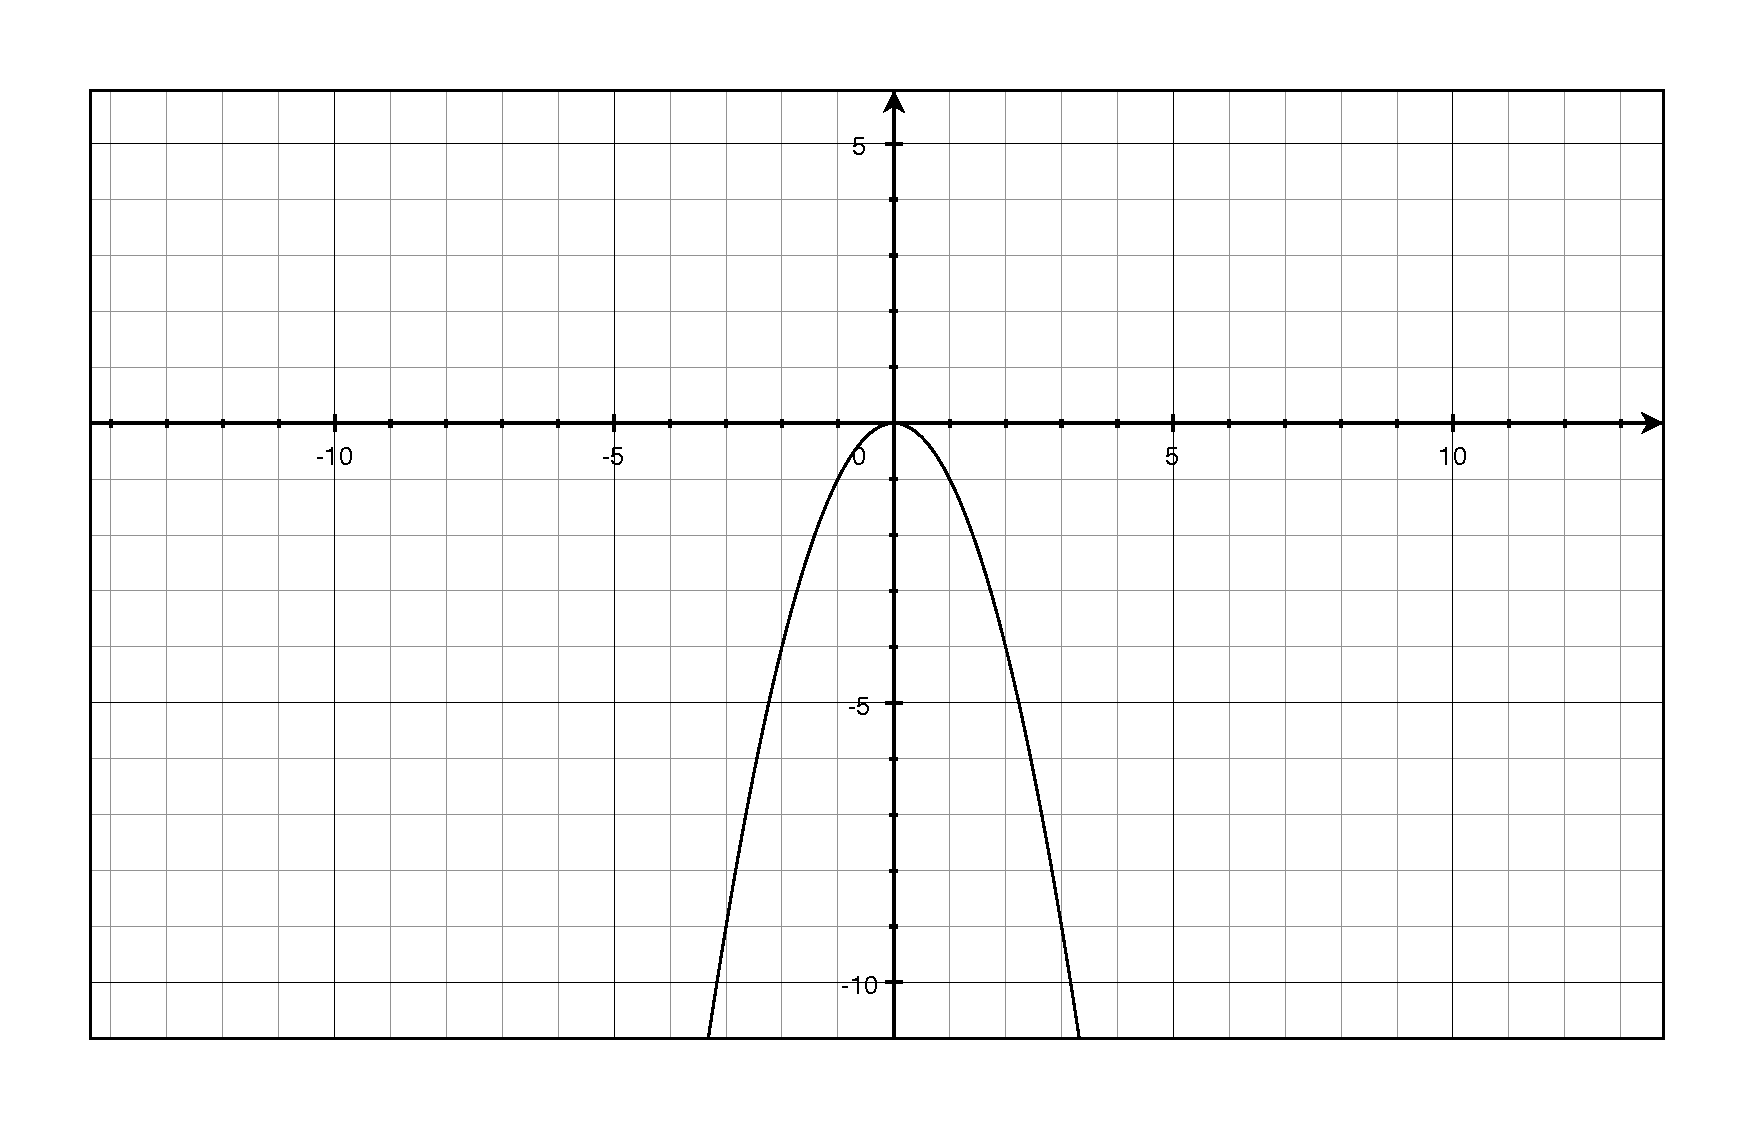
\includegraphics[scale=0.8]{problem7.eps}
  %   \caption*{Problem 7}
  % \end{figure}

  % \begin{tabular}{cc}
  %   \toprule
  %   period & amplitude \\
  %   \midrule
  %   value one & value two
  %   \bottomrule
  % \end{tabular}

  \printanswers

  \ifprintanswers 
    \usepackage{2in1, lscape} 
  \fi

  \date{July 3, 2013}
  \author{}
  \title{Math 141 \\ Homework 17}

  \begin{document}

    \maketitle

    \section{Calendar}
    \begin{itemize*}
      \item July 10: chapter 4 review
      \item July 17: chapter 4 exam
      \item July 24: course review
      \item July 31: final exam
      \item August 21: first day of Math 142 
    \end{itemize*}

    \section{Homework}
    Section 4.5: 1-25, 29-40 

    \section{Extra Credit}
    Section 4.5: 41

    \ifprintanswers
      \begin{description}
        \item[52] TO DO
      \end{description}
    \fi

    \section{Review}

    Find the average rate of change for each function between the given values of the variable (Section 2.3).

    \begin{enumerate}
      \item $f(x) = x^3 - 2x$; $x = -1$, $x = 3$
        \begin{solution}
          \begin{align*}
            f_{avg} &= \frac{3^3 - 2 \cdot 3 - \left( (-1)^3 - 2(-1) \right)}{3 - (-1)} \\
                    % &= \frac{27 - 6 - \left( -1 + 2 \right)}{4} \\
                    % &= \frac{21 - \left( 1 \right)}{4} \\
                    &= 5 \\
          \end{align*}
        \end{solution}

      \item $f(x) = \frac{2}{x + 1}$; $x = a$, $x = a + h$
        \begin{solution}
          \begin{align*}
            f_{avg} &= \cfrac{\cfrac{2}{a + h + 1} - \cfrac{2}{a + 1}}{a + h - a} \\
                    &= \frac{2a + 2 - (2a + 2h + 2)}{h(a + h + 1)(a + 1)} \\
                    &= \frac{2h}{h(a + h + 1)(a + 1)} \\
                    &= \frac{2}{(a + h + 1)(a + 1)} \\
          \end{align*}
        \end{solution}

    \end{enumerate}

  \ifprintanswers
    \section{Section 4.5}

    \begin{description}

      \item[1]
        \begin{enumerate}[a]
          \item \boxed{1.2\%}

          \item $n(3) \approx \boxed{1,929}$

          \item
            \begin{align*}
              10,000 & = 500 e^{0.45t} \\
              t      & \approx \boxed{\unit[6.7]{hr}} \\
            \end{align*}

        \end{enumerate}

      \item[2]
        \begin{enumerate}[a]
          \item $n(0) = \boxed{500}$

          \item $n(5) \approx \boxed{ \unit[12.7]{million\ fish}} $

          \item
            \begin{align*}
              30 & = 12 e^{0.012t} \\
              t      & \approx \boxed{\unit[76]{yr}} \\
            \end{align*}

          \item
            \begin{figure}[H]
              \centering
              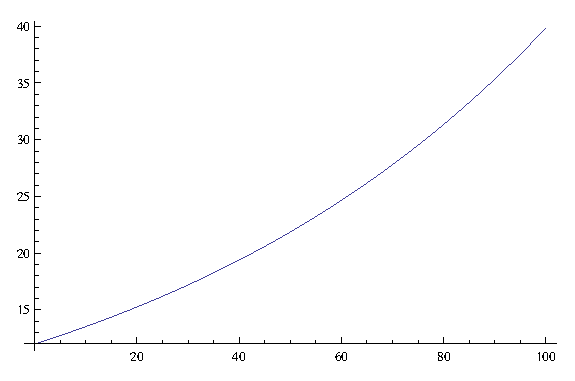
\includegraphics{problem2.eps}
              \caption{Problem 2}
            \end{figure}
        \end{enumerate}

      \item[3]
        \begin{enumerate}[a]
          \item $n(t) = 18,000 e^{.08t}$

          \item $n(8) \approx \boxed{ \unit[34,137]{foxes}} $

          \item
            \begin{figure}[H]
              \centering
              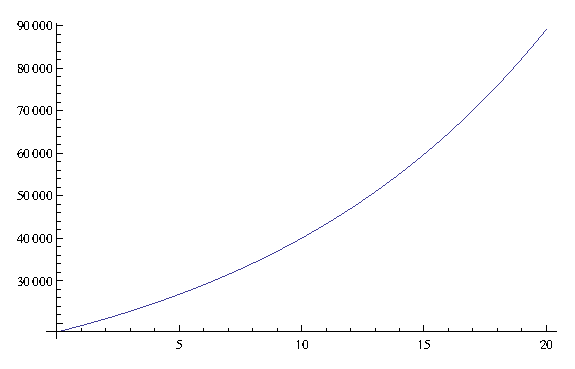
\includegraphics{problem3.eps}
              \caption{Problem 3}
            \end{figure}
        \end{enumerate}

      \item[4] 
        \begin{enumerate}[a]
          \item $n_{2\%}(25) = 110 e^{.03 \cdot 25} \approx \boxed{ \unit[233]{million \ people}}$

          \item $n_{3\%}(t) = 110 e^{.02\cdot 25} \approx \boxed{ \unit[181]{million \ people}}$
        \end{enumerate}

      \item[5] 
        \begin{enumerate}[a]
          \item $n(t) = 112,000 e^{.04t}$

          \item $n(6) \approx \boxed{\unit[142,380]{people}}$

          \item 
            \begin{align*}
              200,000 & = 112,000 e^{.04t} \\
              t       & \approx \unit[14.5]{year} \\
            \end{align*}

            The population will reach 200,000 in the middle of \fbox{2012}. 

        \end{enumerate}

      \item[6] 
        \begin{enumerate}[a]
          \item \fbox{$n(t) = 85 e^{.18t}$}

          \item $n(3) \approx \boxed{\unit[146]{frogs}}$

          \item 
            \begin{align*}
              600 & = 85 e^{.18t} \\
              t   & \approx \boxed{\unit[10.8]{year}} \\
            \end{align*}

        \end{enumerate}

      \item[7] 
        \begin{enumerate}[a]
          \item $n(0) = \boxed{\unit[20,000]{deer}}$

          \item use the other point to find the rate:
            \begin{align*}
              31,000 & = 20,000 e^{4r} \\
              r      & \approx 0.1096 \\
            \end{align*}

            The function is: \fbox{$n(t) = 20,000 e^{0.1096t}$}

          \item $n(8) \approx \boxed{\unit[48,064]{deer}}$

          \item 
            \begin{align*}
              200,000 & = 20,000 e^{0.1096 t} \\
              t       & \approx \unit[21]{year} \\
            \end{align*}

            In \fbox{2017} the population will be 200,000.

        \end{enumerate}

      \item[8] 
        \begin{enumerate}[a]
          \item find the rate:
            \begin{align*}
              2n_0 & = n_0 e^{30r} \\
              2    & =  e^{30r} \\
              r    & \approx 0.02310 \\
            \end{align*}

            The function is: \fbox{$n(t) = 1,500 e^{0.02310 t}$}

          \item 2 hours is 120 minutes.  $n(120) \approx \boxed{\unit[23,986]{bacteria}}$

          \item 
            \begin{align*}
              4,000 & = 1,500 e^{0.02310 t} \\
              t     & \approx \boxed{\unit[42]{minute}} \\
            \end{align*}

        \end{enumerate}

      \item[9] 
        \begin{enumerate}[a]
          \item find the rate:
            \begin{align*}
              10,000 & = 8,000 e^{r} \\
              r      & \approx 0.2231 \\
            \end{align*}

            The function is: \fbox{$n(t) = 8,000 e^{0.2231 t}$}

          \item $n(2) \approx \boxed{\unit[12,499]{bacteria}}$

          \item 
            \begin{align*}
              16,000 & = 8,000 e^{0.2231 t} \\
              t      & \approx \boxed{\unit[3.1]{hour}} \\
            \end{align*}

        \end{enumerate}

      \item[10] 
        \begin{enumerate}[a]
          \item Take the starting point as the time when there were 400 bacteria and find the growth rate:
            \begin{align*}
              400 & = 25,600 e^{4r} \\
              r   & \approx 1.04 \\
                  & = \boxed{104\%} \\
            \end{align*}

          \item 
            \begin{align*}
              400 & = n_0 e^{1.04 \cdot 2} \\
              n_0 & \approx \boxed{\unit[50]{bacteria}} \\
            \end{align*}

          \item \fbox{$n(t) = 50 e^{1.04t}$}

          \item $n(4.5) \approx \boxed{\unit[5,389]{bacteria}}$

          \item 
            \begin{align*}
              50,000 & = 50 e^{1.04 t} \\
              t      & \approx \boxed{\unit[6.6]{hour}} \\
            \end{align*}
        \end{enumerate}

      \item[11] 
        In general, if you want to see when the population will be $x$ times its original size:
        \begin{align*}
          n_0 \cdot x & = n_0 e^{rt} \\
          x           & =  e^{rt} \\
          \ln x       & = rt \\
          t           & = \frac{\ln x}{r} \\
        \end{align*}

        \begin{enumerate}[a]
          \item 
            \begin{align*}
              t & = \frac{\ln 2}{0.02} \\
                & \approx \unit[35]{years} \\
            \end{align*}

            The population will have doubled by \fbox{2020}.

          \item 
            \begin{align*}
              t & = \frac{\ln 3}{0.02} \\
                & \approx \unit[55]{years} \\
            \end{align*}

            The population will have tripled by \fbox{2040}.
        \end{enumerate}
    \end{description}

  \else
    \vspace{1 cm}
    \begin{quote}
      \begin{em}
        \ldots most legislators, politicians, lawyers, ministers, and office-holders serve the state chiefly with their
        heads; and, as they rarely make any moral distinctions, they are as likely to serve the devil, without intending
        it, as God. A very few, as heroes, patriots, martyrs, reformers in the great sense, and men, serve the state with
        their consciences also, and so necessarily resist it for the most part; and they are commonly treated as enemies
        by it.      
      \end{em}
    \end{quote}
    \hspace{1 cm} --Henry David Thoreau
  \fi


  % chomsky:
        % The political policies that are called conservative these days would appall any genuine conservative, if there
        % were one around to be appalled. For example, the central policy of the Reagan Administration---which was
        % supposed to be conservative---was to build up a powerful state. The state grew in power more under Reagan than
        % in any peacetime period, even if you just measure it by state expenditures. The state intervention in the
        % economy vastly increased. That's what the Pentagon system is, in fact; it's the creation of a state-guaranteed
        % market and subsidy system for high-technology production.

        % The ``corporatization of America'' during the past century has been an attack on democracy—and on markets,
        % part of the shift from something resembling "capitalism" to the highly administered markets of the modern
        % state/corporate era. A current variant is called "minimizing the state," that is, transferring decision-making
        % power from the public arena to somewhere else: "to the people" in the rhetoric of power; to private tyrannies,
        % in the real world.

\end{document}

